\section{Multi-Agent Environment Synthesis}
\label{app:synthesis}

\subsection{Admission Checks}

Table~\ref{tab:gates} lists the checks behind the admission decision $f_{\mathrm{gate}}$ of Section~\ref{sec:synthesis}.
A candidate that fails any check is returned to the generator with the failing evidence, and a candidate that cannot be repaired within the generation budget is discarded.
Every attempt starts from a reset environment, so an admitted task never depends on state left by an earlier attempt.

\begin{table}[ht]
\centering\small
\caption{Admission checks and their acceptance conditions. The first three checks are executed by code, and the fourth is a semantic review that reads the request together with the recorded execution evidence.}
\label{tab:gates}
\renewcommand{\arraystretch}{1.15}
\begin{tabularx}{\linewidth}{@{}>{\raggedright\arraybackslash}p{.20\linewidth}Y@{}}
\toprule
Check & Acceptance condition \\
\midrule
Plan validity & Allowed tools, valid arguments, unique call identifiers, and references that resolve to earlier observations. \\
Graph consistency & One node per reference call plus one answer node, acyclic forward edges consistent with the observed execution, and state-order edges supported by an observed state change. \\
Execution and replay & The reference plan executes, the checker accepts the produced answer and database effect, the checker rejects corrupted answers and state, and a replay from a fresh state reproduces both without unexpected mutations. \\
Semantic review & The request is fulfilled, the answer is complete, both parent goals survive, the operations form one coherent task, the state claims agree with the database, and every repeated call serves a distinct purpose. \\
\bottomrule
\end{tabularx}
\end{table}

\subsection{Independence Verification}

Eq.~\ref{eq:pi} records a pair of reference calls as independent only when the graph contains no path between them in either direction, both calls are non-mutating, and the reference plan produces the same answer and the same database effect when the two calls are executed in the opposite order.
The permutation test is run inside a reset environment, and a pair that fails it is dropped from $\Pi$ even when composition proposed it as a parallel branch.
Tasks whose reference contains mutating operations on shared records therefore contribute a small $\Pi$, and the schedule term of Eq.~\ref{eq:sched} is computed over the recorded pairs only.
Section~\ref{sec:abl-reward} reports the fraction of training tasks that carry a verified independent pair.

\subsection{Synthesis Cases}
\label{app:cases}

\begin{figure}[ht]
  \centering
  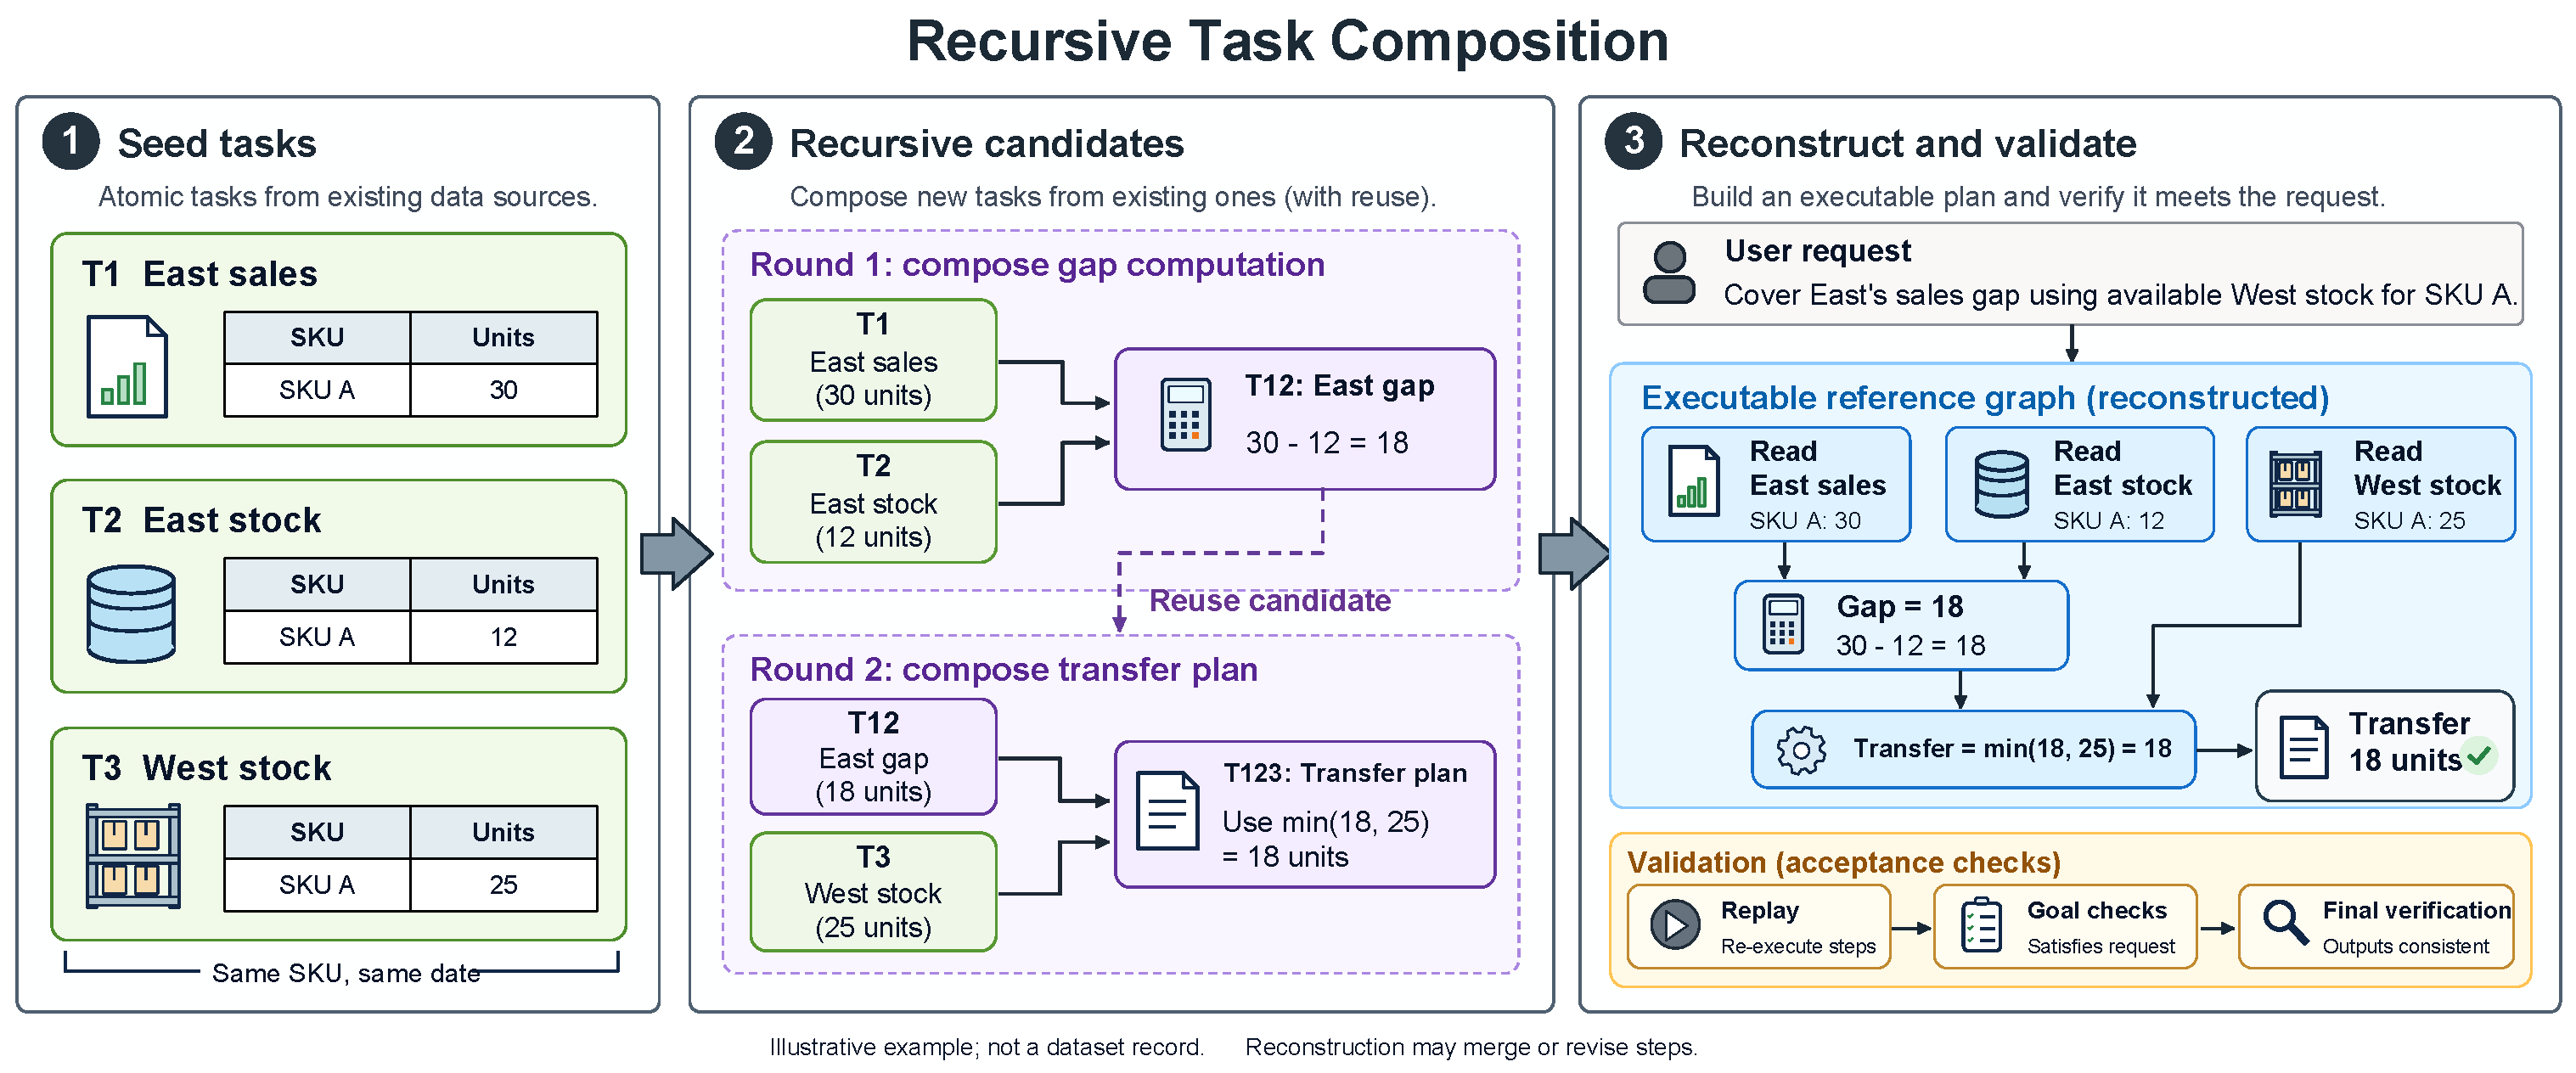
\includegraphics[width=\linewidth]{figures/figure3.pdf}
  \caption{Recursive composition on an illustrative task family. Two rounds of the serial operator turn three atomic seeds into a transfer plan, and reconstruction rebuilds the composed candidate as one executable reference graph that replay and goal checks then validate.}
  \label{fig:composition}
\end{figure}

Figure~\ref{fig:composition} first shows the mechanism on an illustrative task family.
The two cases below show how composition combines parent goals and how reconstruction turns a composed graph into an executable task.
Parent goals and observations are summarized for readability, and the generated request and the reference answer are reproduced in full.

\begin{systembox}{Case 1 \quad Parallel branches over a control plane}
\textbf{Environment.} Control planes with routes and services, and groups of member control planes.

\casepart{Parent tasks and composed graph}
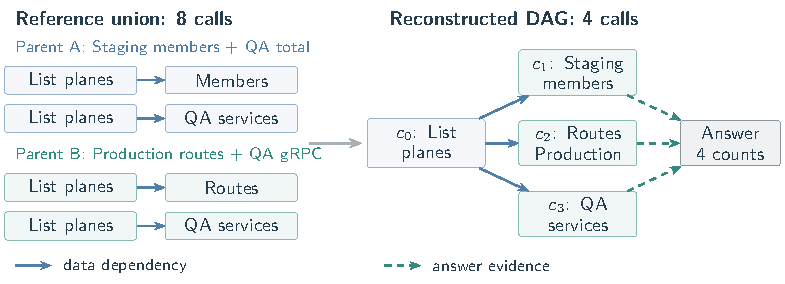
\includegraphics[width=\linewidth]{figures/synthesis_case_kong.pdf}

The two parent graphs form an eight-call reference union. Reconstruction merges the four discovery calls into one and the two service queries into one, and all four requested counts survive.

\casepart{Generated request}
Find the control plane group named 'Staging' and count how many member control planes belong to that group. Then find the control plane named 'Production' with cluster type 'k8s' and count how many routes it has. Next, find the control plane named 'QA' with cluster type 'hybrid' in the 'ap-south' region and count both how many services are deployed to it and how many of those services use the 'grpc' protocol. Return the member count for the Staging group, the route count for Production, the total service count for QA, and the gRPC service count for QA.

\casepart{Reference execution}
\begingroup
\setlength{\tabcolsep}{3pt}\renewcommand{\arraystretch}{1.13}
\begin{tabularx}{\linewidth}{@{}l>{\raggedright\arraybackslash}p{.50\linewidth}Y@{}}
\toprule
 & Tool call & Observation \\
\midrule
$c_0$ & \texttt{list\_control\_planes()} & Staging group 2, Production 1, QA 5. \\
$c_1$ & \texttt{list\_control\_plane\_group\_memberships}\newline\texttt{(groupId=2)} & 2 member planes. \\
$c_2$ & \texttt{list\_routes(controlPlaneId=1)} & 30 routes. \\
$c_3$ & \texttt{list\_services(controlPlaneId=5)} & 10 services, 6 use gRPC. \\
\bottomrule
\end{tabularx}
\endgroup

\casepart{Reference answer and record}
\noindent\begin{minipage}[t]{.60\linewidth}
\vspace{0pt}
\begin{lstlisting}[style=casejson]
{
  "staging_group_member_count": 2,
  "production_route_count": 30,
  "qa_total_service_count": 10,
  "qa_grpc_service_count": 6
}
\end{lstlisting}
\end{minipage}\hfill\begin{minipage}[t]{.36\linewidth}
\vspace{3pt}\raggedright
\textbf{State.} Unchanged.\par\smallskip
\textbf{Independent pairs.} $(c_1,c_2)$, $(c_1,c_3)$, $(c_2,c_3)$, all confirmed by reordered execution.
\end{minipage}
\end{systembox}

\begin{systembox}{Case 2 \quad Serial dependency with pruned calls}
\textbf{Environment.} Documentation sources with crawl, indexing, and search operations.

\casepart{Parent tasks and composed graph}
Parent A refreshes the sources, counts enabled documents, and searches for ``hooks''. Parent B refreshes the same sources, reports enabled documents and index size, and searches for ``error''.

\smallskip
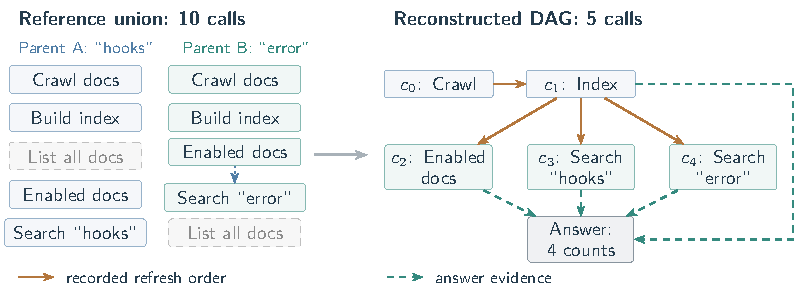
\includegraphics[width=\linewidth]{figures/synthesis_case_docs.pdf}

Reconstruction shares the crawl, the index build, and the enabled-source query, keeps both searches, and removes two listing calls whose outputs support no requested result. The refresh-before-query order is recorded as a state dependency.

\casepart{Generated request}
Refresh the documentation search system by crawling all enabled documentation sources and rebuilding the search index. Then verify the system is working by checking how many documentation sources are currently enabled and indexed, and test the search functionality by querying for both 'hooks' and 'error'. Report the total number of enabled docs, total index entries created, and the number of search results found for each query term.

\casepart{Reference execution}
\begingroup
\setlength{\tabcolsep}{3pt}\renewcommand{\arraystretch}{1.13}
\begin{tabularx}{\linewidth}{@{}l>{\raggedright\arraybackslash}p{.50\linewidth}Y@{}}
\toprule
 & Tool call & Observation \\
\midrule
$c_0$ & \texttt{crawl\_docs()} & Enabled sources crawled. \\
$c_1$ & \texttt{build\_index()} & 10 docs indexed, 224 entries. \\
$c_2$ & \texttt{list\_enabled\_docs()} & 10 docs enabled and indexed. \\
$c_3$ & \texttt{search\_docs(query='hooks')} & 2 matches. \\
$c_4$ & \texttt{search\_docs(query='error')} & 0 matches. \\
\bottomrule
\end{tabularx}
\endgroup

\casepart{Reference answer and record}
\noindent\begin{minipage}[t]{.60\linewidth}
\vspace{0pt}
\begin{lstlisting}[style=casejson]
{
  "enabled_docs_count": 10,
  "index_entries_created": 224,
  "hooks_search_results": 2,
  "error_search_results": 0
}
\end{lstlisting}
\end{minipage}\hfill\begin{minipage}[t]{.36\linewidth}
\vspace{3pt}\raggedright
\textbf{State.} 10 documents updated, 24 pages and 224 index rows added.\par\smallskip
\textbf{Independent pairs.} $(c_2,c_3)$, $(c_2,c_4)$, $(c_3,c_4)$, all after the refresh.
\end{minipage}
\end{systembox}


\section{Dataset Profile and Additional Analyses}
\label{app:stats}



\begin{figure}[ht]
  \centering
  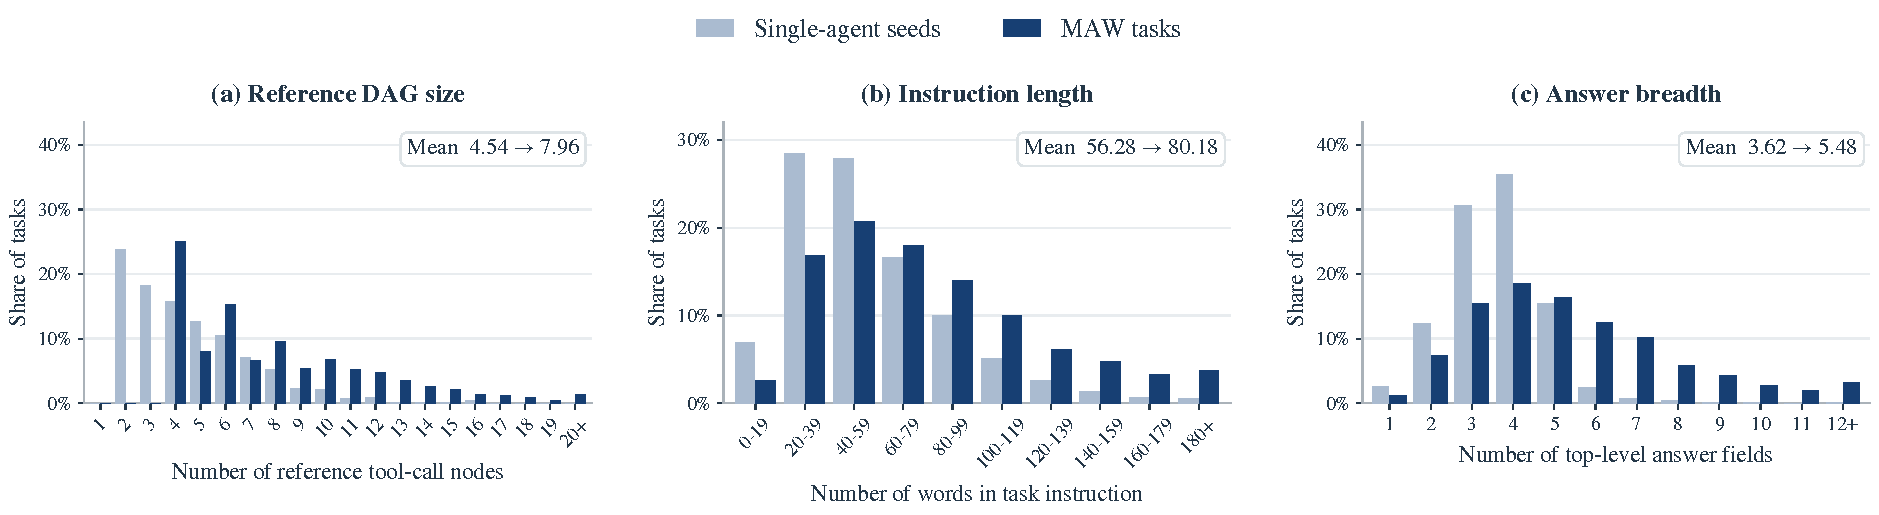
\includegraphics[width=\linewidth]{figures/task_statistics.pdf}
  \caption{Reference structure of the seed pool and of the admitted MAW tasks over 10,860 seeds and 2,581 admitted tasks in 539 environments. Composition grows the number of answer fields far more than the number of tool calls, which indicates that an admitted task asks for more separable results and not simply a longer call chain.}
  \label{fig:task-stats}
\end{figure}

As shown in Figure~\ref{fig:task-stats}, reference tool calls grow by 19.6\% relative to the two parents of each admitted task, distinct tools by 3.9\%, and top-level answer fields by 57.3\%.
The matched baseline of a task is the mean of its two parents, and a parent reused by several descendants contributes once per descendant.

\subsection{Sensitivity, Transfer, and Qualitative Inspection}
\label{app:extra}



\paragraph{Effect of the Process Coefficient and the Schedule Weight.}
\label{sec:sensitivity}

To verify that the reported gains do not depend on a narrow choice of reward weights, we sweep the process coefficient $\lambda$ of Eq.~\ref{eq:reward} and the schedule weight $\alpha_{\mathrm{s}}$ of Eq.~\ref{eq:proc}, keeping every other setting fixed.
The sweep covers the value that removes the process term entirely and values that raise it until process credit approaches the scale of a verified success.

\begin{table}[t]
\centering
\small
\caption{Sensitivity of MAW to the process coefficient $\lambda$ and the schedule weight $\alpha_{\mathrm{s}}$. All rows share the task set, the initialization, and the training budget. The setting used throughout the paper is \colorbox{gray!15}{shaded}.}
\label{tab:sensitivity}
\setlength{\tabcolsep}{6pt}
\renewcommand{\arraystretch}{1.12}
\begin{tabular}{@{}lccc|lccc@{}}
\toprule
$\lambda$ & Success (\%) \up & Goal cov. (\%) \up & $C$ \down & $\alpha_{\mathrm{s}}$ & Success (\%) \up & Goal cov. (\%) \up & $C$ \down \\
\midrule
0.0 & & & & 0.00 & & & \\
0.1 & & & & 0.15 & & & \\
\rowcolor{gray!15}
0.3 & & & & 0.30 & & & \\
0.5 & & & & 0.45 & & & \\
1.0 & & & & 0.60 & & & \\
\bottomrule
\end{tabular}
\end{table}


As shown in Table~\ref{tab:sensitivity}, success is stable across the middle of both ranges and degrades only at the two ends.
A very small $\lambda$ reproduces the outcome-only behavior, and a very large $\lambda$ lets a team collect process credit without finishing the task, which raises goal coverage while success falls.
The schedule weight behaves in the same way, where removing it returns the critical path to the untrained level and raising it too far encourages splitting work that is cheaper to keep together.
The plateau in the middle indicates that the values in Table~\ref{tab:config} were not selected from a narrow optimum.

\paragraph{Generalizability across Worker Backbones.}
\label{sec:worker}

To verify that orchestration training produces a transferable policy and not a policy fitted to one particular worker, we pair the orchestrator trained with frozen Qwen3-8B workers with workers of a different capability at inference and apply no further update.
We keep the interface, the prompts, the budget, and the evaluation instances unchanged, so the only difference is the worker backbone.

\begin{table}[t]
\centering
\small
\caption{Generalization of the trained orchestrator across worker backbones. The orchestrator is trained once with frozen Qwen3-8B workers and then paired with different workers at inference without further updates.}
\label{tab:worker}
\setlength{\tabcolsep}{6pt}
\renewcommand{\arraystretch}{1.12}
\begin{tabular}{@{}llccc@{}}
\toprule
Orchestrator & Workers & Success (\%) \up & $C$ \down & Delivery \up \\
\midrule
Single-agent (init) & Qwen3-8B & & & \\
\rowcolor{gray!15}
MAW & Qwen3-8B & & & \\
Single-agent (init) & Qwen3-14B & & & \\
\rowcolor{gray!15}
MAW & Qwen3-14B & & & \\
\bottomrule
\end{tabular}
\end{table}


As shown in Table~\ref{tab:worker}, MAW improves over the untrained orchestrator under both worker backbones, and the gain in delivery is larger with the weaker workers, where reassignment after an incomplete return matters more.
The critical path shortens under both settings, which indicates that the learned schedule depends on the structure of the request and not on the identity of the worker.
Overall, the results show that the orchestration policy learned in MAW environments carries to teams it was not trained with, which is the property an orchestrator needs in deployment.

\paragraph{Case Study.}
\label{sec:case}

To make the learned behavior concrete, we inspect one successful and one unsuccessful episode from the branch-heavy slice of the held-out set, selected by a fixed sampling rule over the structure of the reference.
In the successful episode, the orchestrator issues one discovery assignment, waits for the identifiers it returns, then assigns three independent lookups in a single concurrent call and merges their results, which matches the dependency and branch pattern that composition wrote into the task.
In the unsuccessful episode, the orchestrator recovers all the branch evidence and drops one of the requested fields when it writes the final answer, which is the integration failure that Eq.~\ref{eq:sched} penalizes and the outcome term alone cannot distinguish from a complete failure.
As shown in Figure~\ref{fig:case}, the two episodes differ only in the final integration step, and the process reward separates them while the outcome term does not.
Appendix~\ref{app:synthesis} provides the full traces, the reference graphs, and the corresponding reward components.

\begin{figure}[t]
  \centering
  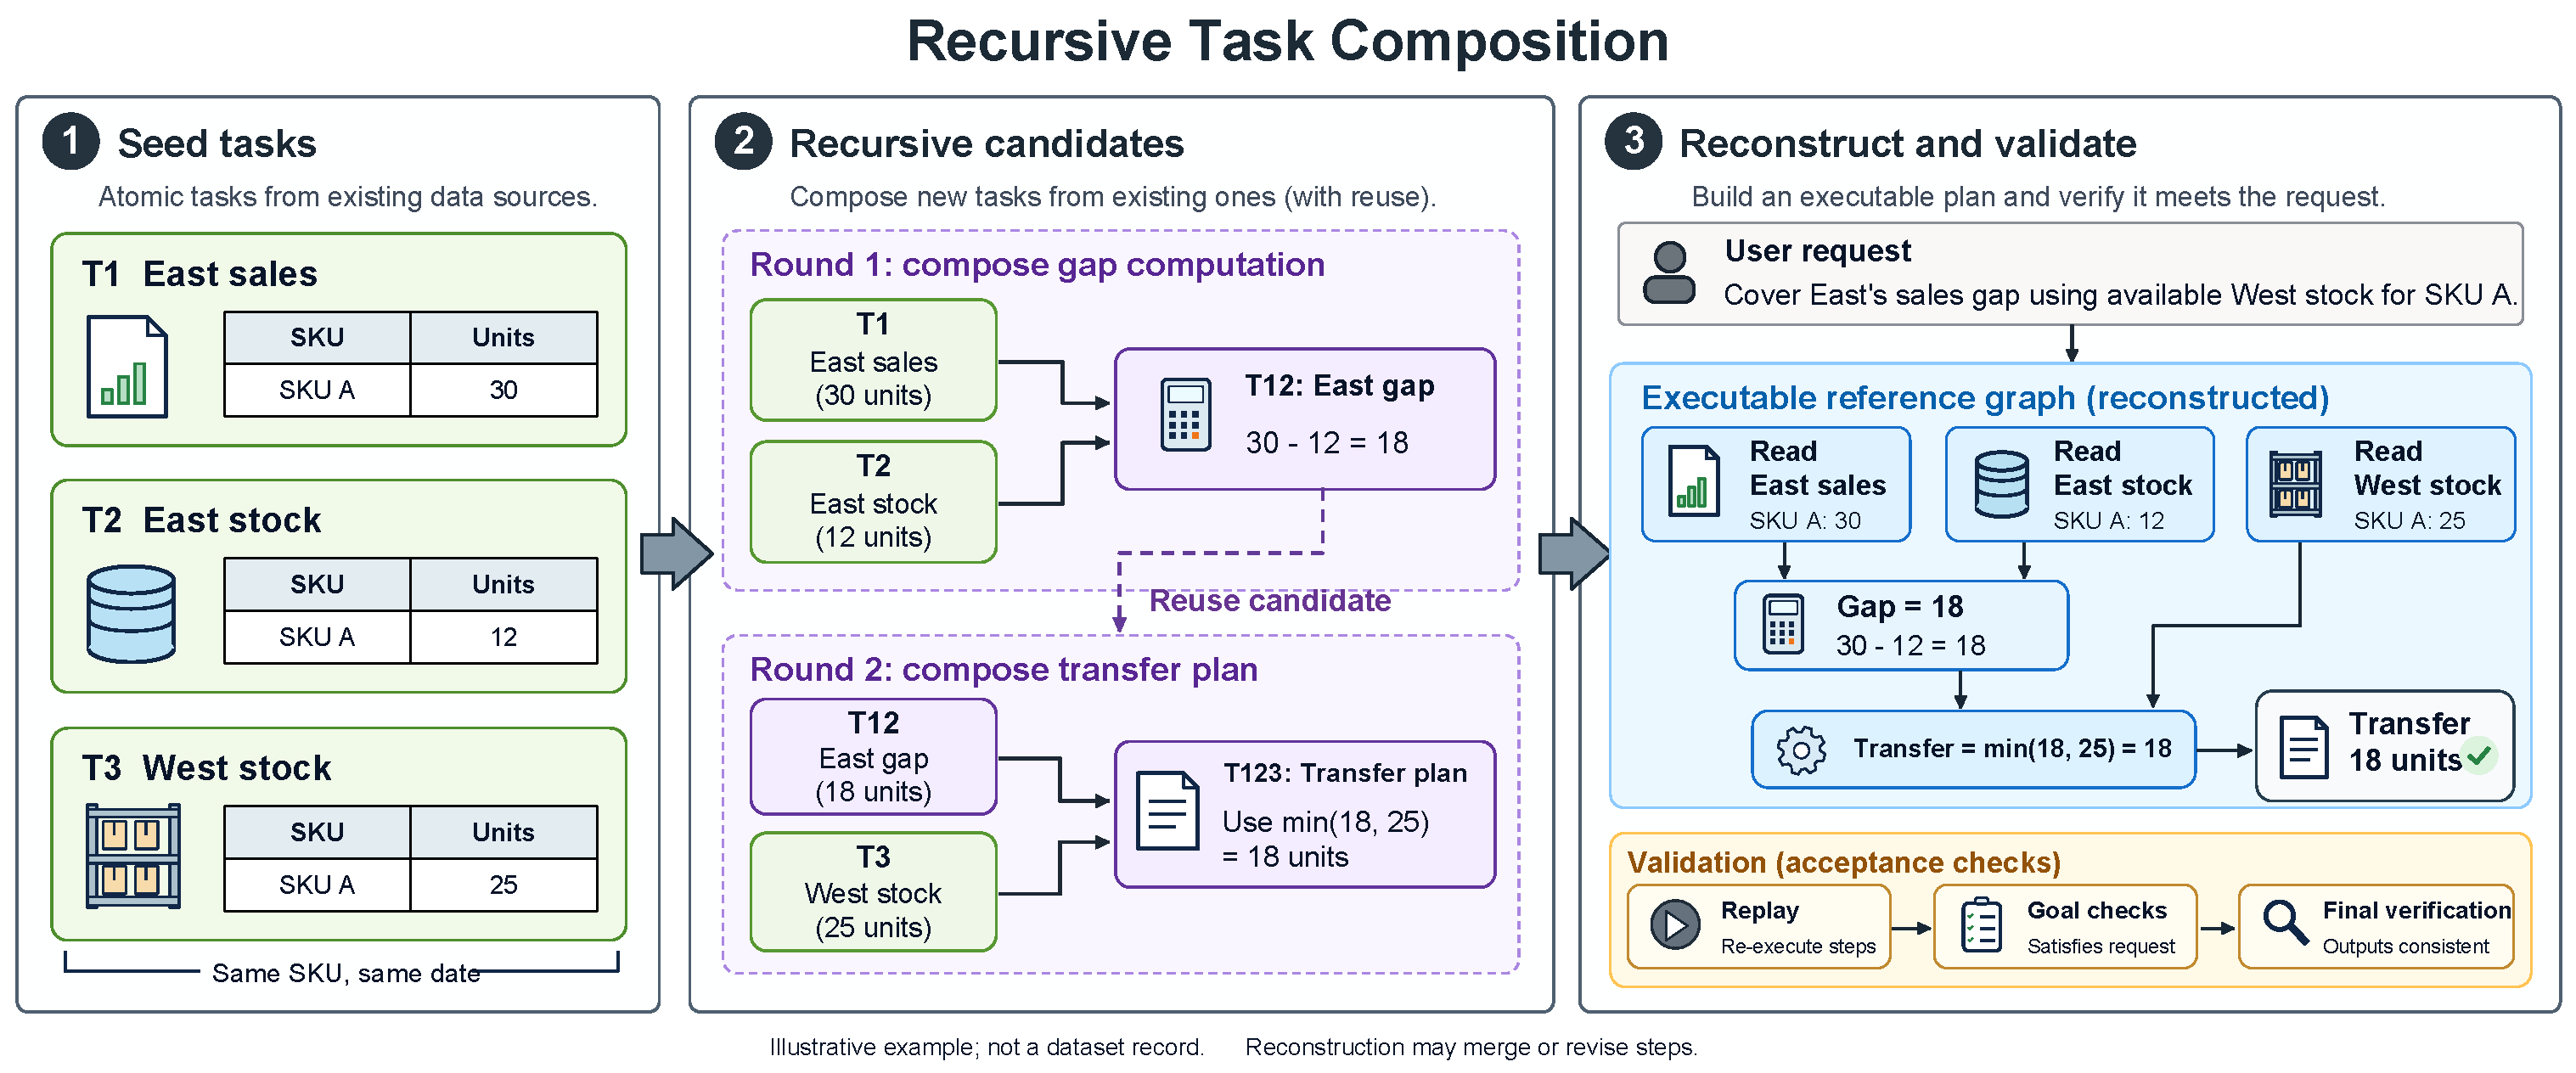
\includegraphics[width=\linewidth]{figures/figure3.pdf}
  \caption{A successful and an unsuccessful episode on the same branch-heavy task. The successful team waits for the discovery result, assigns three independent lookups together, and integrates all of them. The unsuccessful team recovers the same evidence and omits one requested field, which the schedule term penalizes through its integration factor and the outcome term cannot distinguish from a complete failure.}
  \label{fig:case}
\end{figure}

\section{Multi-Agent Runtime and Information Boundary}
\label{app:runtime}

Table~\ref{tab:actions} lists the four actions of the delegation-only harness.

\begin{table}[ht]
\centering\small
\caption{Orchestration interface. A worker is registered with a role and a permitted tool subset, a single assignment is synchronous, and a batch assignment launches workers concurrently and returns when their results join.}
\label{tab:actions}
\begin{tabularx}{\linewidth}{lY}
\toprule
Action & Required information and effect \\
\midrule
\texttt{create\_subagent} & Name, system prompt, and allowed tool names, which registers a worker that follows the frozen policy. \\
\texttt{assign\_task} & Worker name and subtask prompt, which executes one assignment and returns its result. \\
\texttt{assign\_tasks} & A list of assignments, which permits concurrent worker inference and joins the returns. \\
\texttt{submit\_answer} & The final answer in the required format, which triggers completion and verification. \\
\bottomrule
\end{tabularx}
\end{table}

Worker reasoning can overlap, and tool operations on the database commit under a transaction lock, so a concurrent assignment never produces an interleaving that the environment cannot reproduce.
Table~\ref{tab:visibility} states which information each participant can access during an episode.
The reference plan, the expected answer, and the reward components are available only to the reward service, and no reward report is returned to the policy as an observation.
A leakage audit inspects the rendered requests and tool descriptions of the training and evaluation manifests for reference answers, serialized reference graphs, and verifier diagnostics, and tasks descending from the same seed family are grouped before any split.

\begin{table}[ht]
\centering\small
\caption{Information boundary during an episode. Reward reports are never returned as observations, so the policy cannot read its own process score.}
\label{tab:visibility}
\begin{tabularx}{\linewidth}{Yccc}
\toprule
Information & Orchestrator & Worker & Reward service \\
\midrule
User request & Yes & Assigned content & Yes \\
Allowed tool descriptions & Yes & Permitted subset & Yes \\
Tool and worker returns & Returned content & Own context & Logged content \\
Reference plan and expected answer & No & No & Yes \\
Independence record $\Pi$ & No & No & Yes \\
Reward component scores & No & No & Yes \\
\bottomrule
\end{tabularx}
\end{table}

\paragraph{Critical-path Reconstruction.}
Execution cost is a diagnostic and is not part of Eq.~\ref{eq:reward}.
Let $w(v)=1$ for each orchestrator or worker generation event and zero otherwise.
Retaining only causal parents, the depth of an event and the cost of an episode are
\begin{equation}
d(v)=w(v)+\max_{u\in\mathrm{pa}(v)}d(u),\qquad C(\tau)=\max_{v\in G_\tau}d(v),
\label{eq:critical-path}
\end{equation}
where an empty maximum is zero and edges that represent only the serialized commit order are excluded.
For a fork and join execution in which one orchestrator generation precedes two worker branches of length three and five and one integration generation follows, the critical path is $1+\max(3,5)+1=7$ model rounds while serial execution of the same ten generations gives $10$.

\section{Reward Computation}
\label{app:process}

\paragraph{Tool and Answer Matching.}
A reference milestone specifies a tool, its arguments, and the expected observation.
Arguments are compared after declared defaults are filled and after the environment-specific normalization rules listed in the task package are applied, and observations are canonicalized and hashed.
Only successful events contribute coverage, and each milestone is credited once, so repeated calls do not raise $f_{\mathrm{tool}}$.
The answer term is $f_{\mathrm{ans}}(\tau)=\tfrac{m}{n^{\star}}(0.8+0.2\tfrac{m}{n})$, where $n^{\star}$ and $n$ are the reference and submitted field counts and $m$ is the matched count, so recall carries most of the weight and the precision factor removes any gain from padding.
Scalar and structured values require equality, and list elements are matched one to one without reuse.

\paragraph{Delivery and Schedule.}
Each credited subtask has one assignment owner, and a repeated or empty instruction receives no ownership.
Delivery checks whether the worker return contains the required raw evidence or a matching derived result, which is stricter than a claim of completion.
For $f_{\mathrm{sch}}$, a pair in $\Pi$ counts toward $\Pi_\tau$ when the two subtasks are owned by different workers and the assignment intervals are causally independent, so issuing two assignments in sequence and waiting for the first does not count as parallel scheduling.
Tasks with an empty $\Pi$ fall back to a conservative schedule score based on covered milestones, satisfied dependencies, and non-redundant assignments.

\paragraph{Outcome Priority.}
Under Eq.~\ref{eq:reward}, a successful team satisfies $f_{\mathrm{out}}=1$ and $f_{\mathrm{proc}}\ge 0$, which gives $R\ge 1$, and an unsuccessful team satisfies $f_{\mathrm{out}}=0$ and $f_{\mathrm{proc}}\le 1$, which gives $R\le\lambda$.
Every verified success therefore outranks every failure, and the property assumes a correct outcome checker and bounded process terms.

\section{Training and Evaluation Configuration}
\label{app:training}

\begin{table}[ht]
\centering\small
\caption{Training configuration of MAW. The orchestrator and the workers start from the same single-agent checkpoint, and only the orchestrator is updated.}
\label{tab:config}
\begin{tabularx}{\linewidth}{YY}
\toprule
Setting & Value \\
\midrule
Backbone & Qwen3-8B \\
Orchestrator initialization & Single-agent checkpoint \\
Worker initialization and update & Same checkpoint, frozen \\
Optimization & GRPO with outcome and process reward \\
Rollouts per task & 8 \\
Process coefficient $\lambda$ & 0.3 \\
Process weights $(\alpha_{\mathrm t},\alpha_{\mathrm a},\alpha_{\mathrm d},\alpha_{\mathrm s})$ & $(0.25,0.25,0.20,0.30)$ \\
Cost in the training reward & None \\
Completion protocol & At least one delegation \\
\bottomrule
\end{tabularx}
\end{table}

Every benchmark is evaluated with a frozen dataset revision, evaluator commit, subset manifest, and decoding configuration, and function-calling accuracy and task success are reported in separate columns with no average across heterogeneous metrics.
The primary unit of analysis is the task, every method attempts the same instances under paired seeds, and uncertainty is estimated with paired bootstrap resampling of task identifiers.
Infrastructure failures such as an unavailable service are logged separately from a valid trajectory that fails verification, and a rerun uses the same inputs and is counted in the run ledger.
Benchmark tasks and benchmark-derived references are excluded from synthesis, from reward annotation, and from model selection.

\section{Statements}
\label{app:statements}

\paragraph{Reproducibility.}
The research package contains the environment and reset manifests, the task provenance and independence records, the synthesis and admission code, the reward implementation, the prompts, the baseline adapters, the training configurations, and the per-task evaluation logs.
Hidden references are stored separately from the assets visible to a solver.

\paragraph{Ethics.}
Synthetic tool environments can encode unrealistic assumptions or faulty checks, so they are executed in isolated sandboxes and reviewed for copied private data, credential-like strings, and unauthorized external effects before release.
The same orchestration capability that distributes useful work can distribute harmful actions, so deployment requires tool-level permissions and monitoring beyond the training reward.
